%
% Capítulo 1
%
\chapter{Introduction} \label{cap:introduction}

Este é o início do capítulo.

Exemplo de indentação do segundo parágrafo.

%
% Secção 1.1
%
\section{Introduction} \label{sec11}

The goal of this project is to develop a web application that allows the management of surfing athletes. This application is mainly aimed at coaches, but athletes can also access it to view their performance. Coaches will be able to register athletes, log different training sessions (e.g. gym, surf), record competition results, and monitor
performance through interactive charts. This will help them analyze progress and adjust training plans. This project is being developed to meet coaches' need for a more efficient and effective platform, replacing manual registration, which can be time-consuming and difficult to manage as the number of athletes grows. The platform not only saves time but also ensures greater accuracy and accessibility of data, allowing coaches to focus more on their athletes’ development and less on administrative tasks.


%
% Secção 1.2
%
\section{System Requirements} \label{sec12}

%
% Secção 1.2.1
%
\subsection{Functional Requirements} \label{sec121}
\begin{itemize}
\item \textbf{User registration:} Coaches should be able to register by providing a username and password.
\item \textbf{Athlete management:} Coaches should be able to add and remove their athletes. Adding an athlete will only require their name and date of birth.
\item \textbf{Athlete profile:} Coaches should be able to add and view information related to their athletes, such as weight, height, body mass index, and more. Athletes can also view this same information.
\item \textbf{Athletes' training records:} Coaches, through interactive tables and charts, should be able to record and track each athlete's training sessions. Each training session contains different information:
\begin{itemize}
\item \textbf{Surf training sessions:} Sea conditions, maneuvers performed, and a training-related questionnaire completed by the athlete.
\item \textbf{Gym training sessions:} Type of exercise, repetitions, and weight.
\end{itemize}
\item \textbf{Athletes' summaries:} The application should allow, weekly or monthly, summaries so that coaches and athletes can analyze the progress.
\item \textbf{Athletes' competition records:} Coaches can store data from their athletes' competitions, such as the date, location, and score achieved.
\end{itemize}
%
% Secção 1.2.2
%
\subsection{Non-Functional Requirements} \label{sec122}
\begin{itemize}
\item \textbf{User-friendly:} The application should be easy to understand, and therefore, it should have a simple and intuitive user interface.
\item \textbf{Cloud Deployment:} The application will be hosted on a cloud platform to ensure easy access. This will allow users to access the platform from anywhere without needing local installations.
\item \textbf{Tested:} The application must include tests to ensure that all functionalities work correctly.
\end{itemize}

%
% Secção 1.2.3
%
\subsection{Optional Features} \label{sec123}
\begin{itemize}
\item \textbf{PDF Generation:} The application should be able to generate a PDF file with the athlete's summaries, so the coach can interact with the summaries more easily.
\item \textbf{Planning of future training sessions:} In addition to accessing past training sessions, the coach will be able to schedule new training sessions by providing the date and type of training. Athletes will be able to access this information.
\item \textbf{Email notifications:} The application will notify athletes by email if any training session is scheduled or changed. For this, athletes will need to associate their email address.
\end{itemize}


%
% Secção 1.3
%
\section{Risks} \label{sec13}
\begin{itemize}
\item Having no knowledge of surfing practice may lead to difficulties in creating a practical design for coaches, as we don’t know the best way to present information to them. Consequently, frequent communication with the practitioners will be essential.
\item In frontend development, we may encounter more challenges because, although these technologies aren't new to us, we have less experience with TypeScript and React.
\end{itemize}

%
% Secção 1.4
%
\section{Plan} \label{sec14}
\begin{figure}[h]
\centering
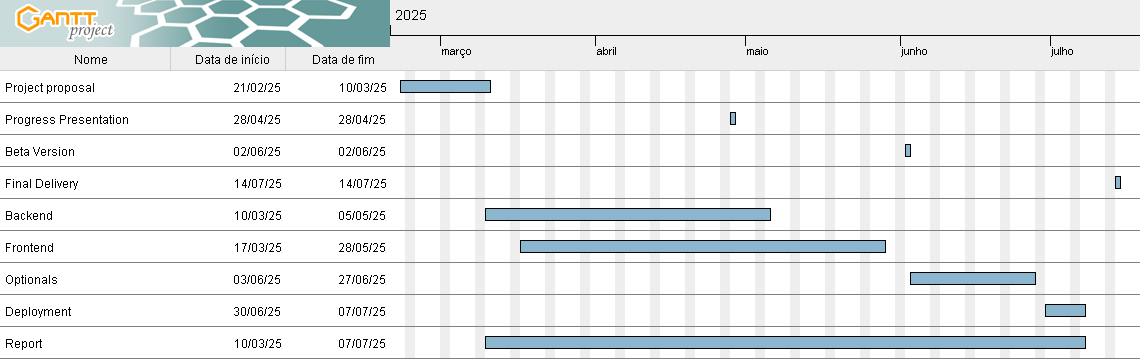
\includegraphics [width=6in]{./figures/GanttChart.png}
\caption{Gantt Chart plan.}
\end{figure}